\title{Spark Execution on Fact Checking and Related Workloads}
\author{
        Brett Walenz \\
        Chaoren Liu\\
}
\date{}
\documentclass[11pt]{article}
\usepackage[parfill]{parskip}
\usepackage[dvipsnames]{xcolor}
\usepackage{geometry}
\usepackage{amsfonts}
\usepackage[mathscr]{eucal}
\usepackage{amsmath}
\usepackage{amssymb}
\usepackage{pgfgantt}
\usepackage{listings}
\usepackage{graphicx}
\usepackage{caption}
\usepackage{subfig}
\usepackage{adjustbox}

\lstset{frame=tb, 
language=Python,
showstringspaces=false,
numbers=none,
breaklines=true
breakatwhitespace=true,
tabsize=4,
aboveskip=3mm,
belowskip=3mm,
columns=flexible,
basicstyle={\small\ttfamily},
numberstyle=\tiny
}

\begin{document}
\maketitle
\section{Overview}
The goal of this project was to gain insight into aspects of the Spark execution engine. In particular, we wished to gain insight into the effect different execution plans has on the overall running time, bandwidth required, and computation time across the cluster. Our task is a computation-heavy task derived from computational fact-finding\cite{cohen2011computational}, where the goal can be thought of as minimizing or maximizing the result of an aggregate query under varying parameters. We'd like to answer the following question:

Which two congressional representatives had the lowest voting agreement percentage with a span of at least 120 days, after January 1st 2012?

\section{Dataset}
The dataset is a collection of congressional voting records from GovTrack.us after January 1st, 2012, consisting of 2770 bills and approximately 900,000 individual votes. The data is initial in an SQL database, but we've denormalized the data to have the following structure:

\begin{table}[h!]
\begin{adjustbox}{max width=\textwidth}
\begin{tabular}{ | l | c | c | c | c | c | c | c | r | }
\hline
Bill Id & Rep Id & Vote & Type & Chamber & Year & Date & Result & Name\\
\hline
h81-113.2013 & A000361 & Yea & procedural & h & 2013 & 2013-03-19 & Passed & Rodney Alexander\\
h81-113.2013 & B001256 & Yea & procedural & h & 2013 & 2013-03-19 & Passed & Michele Bachmann\\
h81-113.2013 & B001279 & Nay & procedural & h & 2013 & 2013-03-19 & Passed & Ron Barber\\
\hline
\end{tabular}
\end{adjustbox}
\end{table}


\section{Approaches}
A very basic approach for finding the vote correlation between representatives is the following. We first parse the votes and key them by billId. We then self-join, and transform the data into (agree, disagree) tuples. The last stage, reduceByKey, sums the number of times two people agree and disagree.  

\begin{lstlisting}
   votes = load_votes(context)
   votes = votes.map(parseVote)
   joined = votes.join(votes)
   counted = joined.map(count_votes)
   counted = counted.reduceByKey(reduce_count)
\end{lstlisting}

This approach finds the vote correlation between all pairs of congressional representatives, but it doesn’t consider the interval of comparison. 

\subsection{A Note on Intervals}
We need a way then, to construct interval sets, which consist of a collection of intervals. For instance, a set of intervals might be exhaustive:
[(1/1/2011, 12/31/2011), (1/2/2011, 12/31/2011), …
(1/1/2011, 1/30/2011), (1/2/2011, 1/30/2011),...
(12/01/2011, 12/31/2011), (12/02/2011, 12/31/2011)]

The above set contains all possible intervals from January 1st, 2011 to December 31st, 2011. The interval contains approximately d(d-1)/2 intervals, or 66300 intervals for just one year. We can obviously reduce this set of intervals by noting many intervals contain the same data, or no data at all. And many intervals may be too small for our condition (spanning 100 votes). Thus, each interval in the set must span at least 120 days. We used the Pandas Python data analysis library for this task\cite{mckinney2012python}.

\subsection{Approach 1 - All in One Shot}

A naive expanded approach may then be something such as:

\begin{lstlisting}[caption={Naive approach}, label={lst:naive-listing}]
   votes = load_votes(context)
   votes = votes.map(parseVote)
   intervals = create_interval_set(start, end, parameters)
   intervals = intervals.filter([100 votes, no empty data, identical sets])
   joined = votes.join(votes)
   joined = joined.cartesian(intervals)
   joined = joined.filter((votes not in each interval))
   counted = joined.map(count_votes)
   counted = counted.reduceByKey(reduce_count)
\end{lstlisting}

The algorithm is a fairly `traditional' Spark approach. We parse each vote line into a $(billid, (values))$ representation, self-join the bills, and cartesian join the interval set. It’s important to note that the above algorithm might be exceedingly large due to the cartesian join performed. Then we map the votes and construct a new key that looks similar to: $entity_a:entity_b:start:end$. 

\subsection{Approach 2 - Interval Iterations}
Listing \ref{lst:iterative-listing} is similar to Listing \ref{lst:naive-listing}, but instead of performing a cartesian join we iterate over the interval set. In this approach, we don't create new keys of the form $entity-a:entity-b:start:end$, instead we store a map on the drive that holds the lowest vote percentage for an original key $entity-a:entity-b$.


\begin{lstlisting}[caption={Iterative approach}, label={lst:iterative-listing}]
    interval_map = dict()
    for (id, start, end) in intervals:
      func = partial(filter_by_int, start=start, end=end)
      temp = counted.filter(func)
      results = temp.reduceByKey(reduce_count)
      results = results.filter(filter_count)
      result_list = results.collect()
      """ Store the lowest result in a dictionary. """
      for result in result_list:
        (key, (agree, disagree, pct)) = result
        if pct_map[key] > pct:
          pct_map[key] = pct
          interval_map[key] = result
\end{lstlisting}

\subsection{Approach 3 - Grouped Key Computations}
We can note that keys of the form $entity-a:entity-b$ have a fairly small number of values: the number of shared votes the two representatives have. If our interval set is also fairly small, we can perform this computation in one batch on a single node without worrying about memory. 


\begin{lstlisting}[caption={Grouped approach}, label={lst:grouped-listing}]
    raw_votes = load_votes(context)
    big_intervals = interval.interval_set('1/1/2012', '1/1/2014', freq='15D',   max_delta=pandas.Timedelta(days=120))
    bills = raw_votes.map(keyByBillId)
    joined = bills.join(bills, 128)
    joined = joined.filter(filter_join)
    counted = joined.map(count_votes)
    big_ints_rdd = context.parallelize([big_intervals], 1)
    grouped = counted.groupByKey(128)
    int_grouped = grouped.cartesian(big_ints_rdd)
    results = int_grouped.map(calculate_percent_grouped)
\end{lstlisting}

Listing~\ref{lst:grouped-listing} does exactly as described. The first part of the algorithm is the same as the first two approaches: self-join the bills, and emit a key, (1, 0, date) if the vote agrees, and a key, (0, 1, date) if the votes do not agree. Next, we parallelize our intervals so they are all within one array and one partition, and then we group the counted votes by key. Then we cartesian the intervals with the grouped data, producing a data set with a rough schema:

\begin{lstlisting}[caption={Schema of grouped function}, label={lst:schema}]
[(key, list(agree, disagree, date)), list(start_date, end_date)]
\end{lstlisting}

\begin{lstlisting}[caption={Grouped percent function}, label={lst:group-function}]
def calculate_percent_grouped(((key, counts), intervals)):
  low = 1
  for id, start, end in intervals:
    total_a = 0
    total_d = 0
    pct = 1
    for agree, disagree, d in counts:
      if d >= start and d <= end:
        total_a += agree
        total_d += disagree
    if total_a == 0 and total_d == 0:
      total_d = 1
    pct = total_a / float(total_a  + total_d)
    if pct < low:
      low = pct
      low_tuple = (start, end, total_a, total_d)
  return (key, low_tuple)
\end{lstlisting}

Listing~\ref{lst:group-function} shows the worker function performed by the slaves. Every key has a collection of (agree, disagree, date) values, and a set of intervals. Then we iterate through the intervals and for each interval calculate the vote correlation. If it's the new low, save it as such.

\section{Experiments}
We tested our approaches on a 5 node Amazon EC2 cluster running Spark 1.2.0. Each EC2 instance was an m3.2xlarge, which is an 8 vCPU, 30 GiB machine, and 2 x 80 GB SSD's, although these weren't used during the runs. The voting file is an uncompressed text file with size 250 MB, consisting of roughly 1000 representatives between the House of Representatives and Senate. The number of joins resulting from this is approximately 130,000, and the number of intervals analyzed was 364, or about $47 \times 10^6$ distinct computations.

\begin{figure}[h!]
\centering
\begin{tabular}{ |c|c|c| }
\hline
\multicolumn{3}{|c|}{Runtime (minutes)}\\
\hline
Naive & Iterative & Grouped\\
\hline
32 & 47 & 7\\
\hline
\end{tabular}
\caption{Overall runtime}
\label{runtime}
\end{figure}

The iterative approach is the slowest approach, and if we examine the Ganglia report from the run we can quickly see why. 

\begin{figure}[h!]
\centering
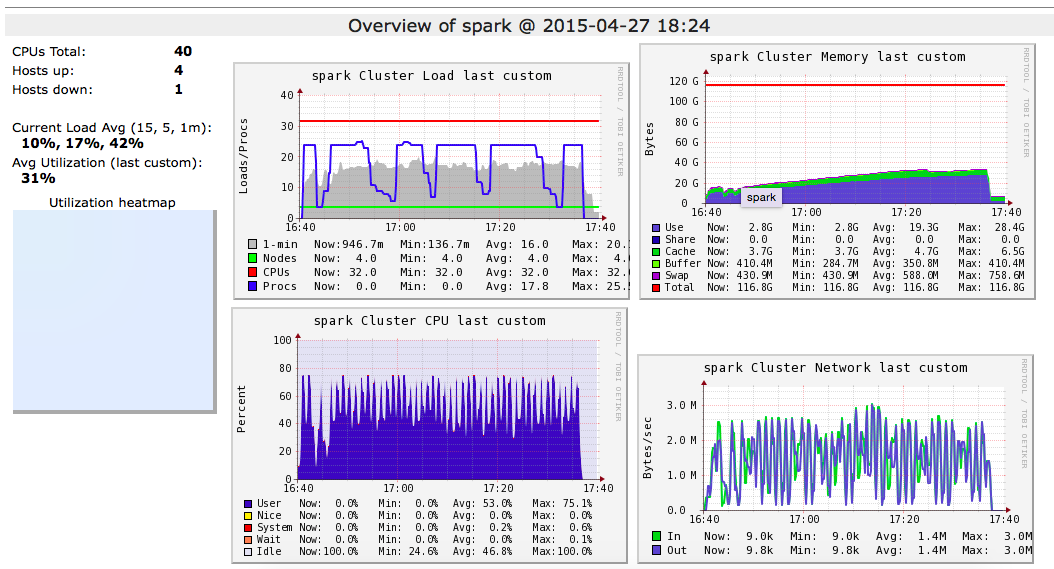
\includegraphics[width=0.8\textwidth]{ganglia_iterative}
\caption{Ganglia display for iterative approach}
\label{fig:ganglia-iterative}
\end{figure}

In Figure \ref{fig:ganglia-iterative}, we can see the bursty nature of both the CPU and bandwidth. Overall CPU utilization was only 31\%, and cluster bandwidth was relatively high with an average of 1.4 MB/sec. The iterative approach induces this type of behavior because every iteration incurs overhead on starting a new set of Spark jobs, while at the end of each iteration a $collect()$ is called, incurring a high bandwidth cost at each iteration. 

The so-called Naive approach performs better and we see much higher CPU utilization overall. However, we assert that the bottleneck in this case is the network overhead incurred at the end of the job: approaching 50MB/sec. The reason for this is that we create an extremely dense set of keys of the form $entity:entity:start:end$, which as noted can be quite large. So a very large shuffle occurs in order for the reduceByKey to function, and then the results from that can be collected.

\begin{figure}[h!]
\centering
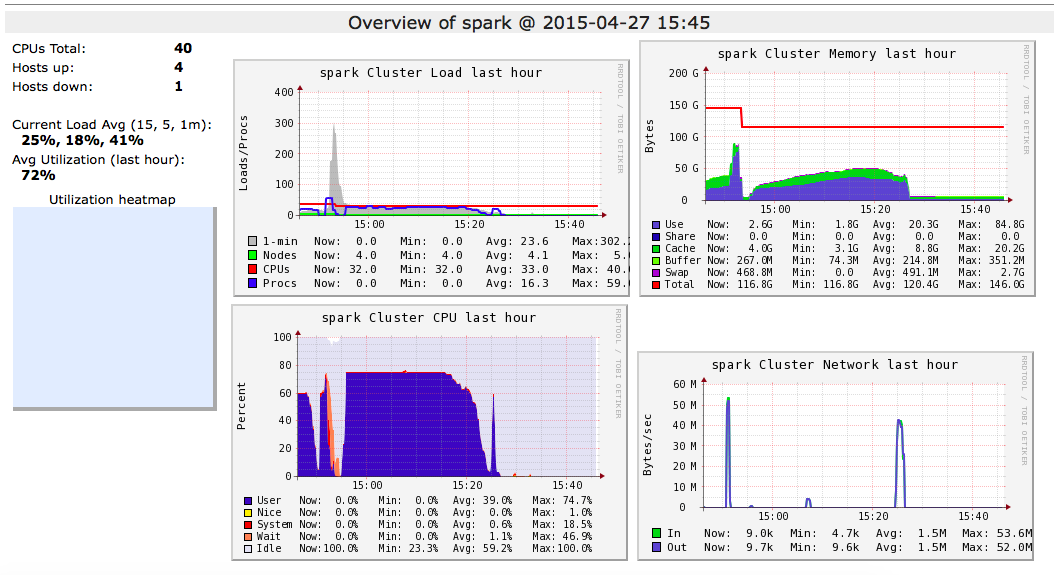
\includegraphics[width=0.8\textwidth]{ganglia_naive}
\caption{Ganglia display for naive approach}
\label{fig:ganglia-naive}
\end{figure}


This led to the third approach with the realization that each computation isn't that expensive: summing the agree and disagree votes for each interval is a straightforward process as long as the data is within one node and we can iterative over the data. In addition, we save almost the entirety of the shuffle from the Naive approach since we calculate the minimum for a key on a node, and send only the min back to the driver. 

\begin{figure}[h!]
\centering
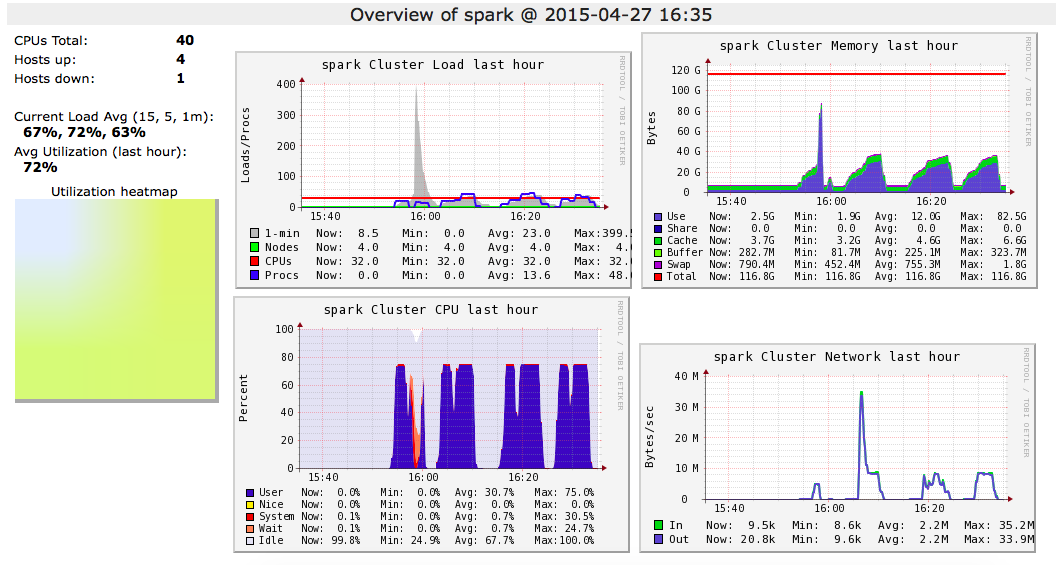
\includegraphics[width=0.8\textwidth]{ganglia_grouped}
\caption{Ganglia display for grouped approach}
\label{fig:ganglia-grouped}
\end{figure}

Figure~\ref{fig:ganglia-grouped} is actually the display of multiple runs, since each run was under 8 minutes. We can see that while active, the grouped approach has roughly the same CPU utilization as the Naive approach but overall uses less memory. This is because we are performing a cartesian in chunks, rather than row by row, resulting in a lot less duplication. 

In the end, the grouped approach closely resembles traditional parallel computing concepts, but it's impressive the ease with which Spark supports this use case. The only drawback to this approach is that we have to be explicitly aware of the size of the work being performed, as we can overload a nodes memory if a collection is too large (be it a key collection or the set of intervals). 

Lastly, a note about data analytics and performance. A recent paper, \textit{Making Sense of Performance in Data Analytics Frameworks}\cite{ousterhoutmaking} discussed some counter-findings to the accepted mantras about commmon performance pitfalls in data analytics. However, in our case our data was small enough that we were able to drastically change the algorithm since we had more flexibility in memory availability. It should be noted, however, that the very existence of the grouped approach is because of the extreme slowness of the reduceByKey and shuffle in the Naive approach. There may be some space where small data, large computation workloads can be optimized in similar fashion.

\section{Conclusion}
In this project, we examined three different approaches to the problem of finding vote correlation among United States congressional representatives. We noticed that a grouped approach was the quickest, and leveraged the fact that the values for each key were relatively small, meaning we could fit everything onto one machine and perform all computation at a node, avoiding expensive shuffles and repartitionings. 

\bibliographystyle{abbrv}
\bibliography{research}

\appendix
\section{Code}
All the code for this project can be found at: https://github.com/bwalenz/cs516-team. We've included the code for the grouped approach, but have omitted the others for brevity. 
\section{Grouped Approach Code}
\begin{lstlisting}[language=Python]
from pyspark import SparkContext
from functools import partial
from collections import defaultdict
import StringIO
import csv
import datetime
import permute.interval as interval
import pandas
import numpy as np
import sqlite3

votes_file = '2012-curr-full-votes.csv'
#master = "local[4]"
master = "spark://ec2-54-83-184-241.compute-1.amazonaws.com:7077"
def load_votes(context):
    votes_data = context.textFile(votes_file, use_unicode=False).cache()
    return votes_data


def keyByBillId(line):
    """
    Key by the bill id to be used in the self join step. The tuple looks like:
    (bill_id, (person_id, date, vote))
    """
    df = '%Y-%m-%d'
    input = StringIO.StringIO(line)
    reader = csv.reader(input)
    tup = reader.next()
    if tup:
      tup[6] = datetime.datetime.strptime(tup[6], df).date()
    reduced = []
    #person id
    reduced.append(tup[1])
    #date
    reduced.append(tup[6])
    #vote (yay, nay, etc)
    reduced.append(tup[2])
    return (tup[0].strip(), [tup[1].strip(), tup[6], tup[2].strip()])

def count_votes((key, joined_tuple)):
    """
    Map function that counts the votes between two entries.
    Called on a self-joined bills entry, so the incoming tuple looks like:
    (bill_id, ((person_id, date, vote), (person_id, date, vote))
    """
    left = joined_tuple[0]
    right = joined_tuple[1]
    left_id = left[0]
    right_id = right[0]
    key = left_id + ":" + right_id
    agree = 0
    disagree = 0
    if left[2] == right[2]:
        agree = 1
    else:
        disagree = 1
    return (key, (agree, disagree, left[1]))


def reduce_count(left, right):
    agree = left[0] + right[0]
    dis = left[1] + right[1]
    return (agree, dis)


def filter_count((key, (agree, dis))):
    """
    Filter any entries that don't have at least 50 votes.
    This is also needed because some entries get filtered out completely
    and so the previous reduce_count stage is not called for some tuples,
    resulting in the third entry in this tuple being a date object instead
    of a percent.
    """
  
    if agree + dis < 50:
        return False
    else:
        return True


def filter_join((key, (left, right))):
    """
    Avoids duplicate calculations/entries
    ex: ("p_id_1:p_id_2", "p_id_2:p_id_1"), removes the right one.
    """
    if left[0] < right[0]:
        return True
    return False

def calculate_percent_grouped_2(((key, counts), intervals)):
  low = 1
  for id, start, end in intervals:
    total_a = 0
    total_d = 0
    pct = 1
    for agree, disagree, d in counts:
      if d >= start and d <= end:
        total_a += agree
        total_d += disagree
    if total_a == 0 and total_d == 0:
      total_d = 1
    pct = total_a / float(total_a  + total_d)
    if pct < low:
      low = pct
      low_tuple = (start, end, total_a, total_d)
  return (key, low_tuple)

def run(context):
    """ Data is in the following format: (bill_id, person_id, vote, type, chamber, year, date, session, status, extra).
        1. Key everything by bill_id, parse the date correctly, return (bill_id, (person_id, vote, date))
        2. Self join bills RDD to itself.
        3. Remove duplicate entries (via left.person_id < right.person_id) and comparisons with self.
        4. Map the joined data to a (person_id:person_id, (agree, disagree)) RDD.
        5. Grouped all the counts by key into one array and partition. 
        6. Cartesian join the intervals.
        7. Run the grouped computation function on each group. 
    """
    raw_votes = load_votes(context)
    big_intervals = interval.interval_set('1/1/2012', '1/1/2014', freq='15D', max_delta=pandas.Timedelta(days=120))
    bills = raw_votes.map(keyByBillId)
    joined = bills.join(bills, 128)
    joined = joined.filter(filter_join)
    counted = joined.map(count_votes)
    big_ints_rdd = context.parallelize([big_intervals], 1)
    grouped = counted.groupByKey(128)
    int_grouped = grouped.cartesian(big_ints_rdd)
    results = int_grouped.map(calculate_percent_grouped_2)

    return results

if __name__ == "__main__":
    context = SparkContext(master, "Congress Correlation")
    results = run(context).collect()
    with open('output.csv', 'w') as csvfile:
      writer = csv.writer(csvfile)
      for result in results:
        (persons, (start, end, agree, disagree)) = result
        person_split = persons.split(":")
        writer.writerow([person_split[0], person_split[1], str(start), str(end), str(agree), str(disagree), str((agree / (agree + disagree)))])
\end{lstlisting}

\end{document}